%Note that he official definitions of University grades has changed
%since this was written
%
%Provided by Carl Lee.

\documentclass[12pt]{article}
\setlength{\oddsidemargin}{0in}
\setlength{\evensidemargin}{0in}
\setlength{\textwidth}{6.5in}
\setlength{\parindent}{0in}
% \setlength{\parskip}{\baselineskip}
\usepackage{graphicx}
\usepackage{multirow}

\usepackage{amsmath,amssymb,amsrefs}

\usepackage[top=24mm, bottom=18mm, left=15mm, right=13mm]{geometry}

\usepackage{url}

\begin{document}


\begin{center}
{\bf Homework 1}\\
{\bf MATH 191 Topics in Data Science}\\
{\bf Posted: October 3, 2015}\\
{\bf Due in class, Friday, October 16} \\
\end{center}

All problems are worth 10 points, except the programming assignment problem which is worth 30 points.

(1)  Recall that the sample covariance of two vectors 
$x,y \in \mathbb{R}^n$ is given by 

$$ cov(x,y)=\frac{1}{n-1} \sum_{i=1}^{n} ( x_i - \bar{x})( y_i - \bar{y})$$
and the sample correlation coefficient is defined as
\begin{equation}
	 cor(x,y) = \frac{cov(x,y)}{\sigma_x \sigma_y}
	 \label{def:corr}
\end{equation}
where $\sigma_x$ and $\sigma_y$ are the sample standard deviations.

(a) Show that the following identify holds
$$ var(x+y) = var(x) +  var(y) + 2 cov(x,y) $$

(b) Using properties of the variance and equation (\ref{def:corr}) show that $\rho \geq -1$.

(c) What is the relationship between the points $(x_1, y_1), \ldots, (x_n,y_n)$ if $\rho = -1$ ?

\vspace{6mm}


(2) Denote by $X_1$ and $X_2$ two independent standard normal random variables. Define new random variables $Y_1,Y_2$ given by
$$ Y_1 = 3 X_1 + X_2, \;\;\;\;  \mbox{ and } Y_2 = X_1 - X_2 $$

(a) Compute $\mathbb{E}[Y_1]$ and $\mathbb{E}[Y_2]$. \\
(b) Compute the covariance $Cov(Y_1,Y_2)$. \\
(c) Find the joint probability density function of $(Y_1,Y_2)$. \\

\vspace{6mm}

(3)  Denote by $X_1$ and $X_2$ two independent normal random variables with the same variance. Define new random variables $Y_1,Y_2$ given by
$$ Y_1 = X_1 - X_2, \;\;\;\;  \mbox{ and } Y_2 = X_1 + X_2 $$
Show that $Y_1$ and $Y_2$ are independent.

\vspace{6mm}


(4) Let $X$ and $Y$ denote two random variables, with finite second moments $\mathbb{E}[X^2]$ and $\mathbb{E}[Y^2]$. \\ 

(a) Show that $ \left( \mathbb{E}[XY] \right)^2  \leq \mathbb{E}[X^2] \; \mathbb{E}[Y^2]$. \textit{Hint: define first $ h(t) = \mathbb{E}[ (X + tY)^2 ] $, consider the sign of this quadratic polynomial in $t$, and remind yourself of the discriminant of a quadratic equation (from middle school).} \\
 
(b) Use (a) to show that the population correlation coefficient $\rho \in [-1,1]$ 
 

\clearpage
 
\textbf{Programming Assignment (30 points)}

Use the provided R script to grab data from Yahoo finance, for a number of financial instruments
$\{ \mbox{'SPY','\^{}VIX','\^{}TNX', 'OIL','GLD','GOLD','\^{}N225','\^{}FTSE','SPXS','SPXL'} \}$. 
In class, we will briefly go over what they represent, though it is not hard to guess or find out what they mean.

\vspace{3mm}

Let $P$ denote the prices matrix, of size $T \times n$, where $T$ is the number of days in history, and $n$ is the number of instruments.  For each time series of a given instrument, compute the so called log-returns
	$$ R_i(t) = log( R_i(t)/R_i(t-1) ) $$
You can do so, for all instruments at once, in R via the command
$$R = \log( P[2:T, ] / P[1:(T-1),])$$

1) Plot a histogram of the returns, for each of the ten instruments.

\vspace{3mm}

2) Compute the sample mean and variance of the return, for each instrument. 

\vspace{6mm}

Next, we will be computing various measures of correlation between the above instruments, namely the following six different correlation measures:  Spearman, Hoeffding, Maximal Correlation, dCor, and MIC.

Here are some useful tips to keep in mind when implementing this in R:

\begin{itemize}
\item Spearman and Pearson correlation (standard)
\item maximal correlation: \textit{library(acepack)} d(the corresponding R package).  Note that you first need to compute \textit{q = ace(x,y)}, and then the maximal correlation via \textit{cor(a\$tx, a\$ty)}. Note that you cannot do this for all pairs of variables at once, but sequentially for each instruments versus everyone else, i.e., run q = ace(R,R[,i]); and do so for for every column  $i=1,\ldots,8$
\item Hoeffding's D:  \textit{library(Hmisc); hoeffd(R)\$D}  returns the entire correlation matrix
\item distance correlation: \textit{library(energy)}; using \textit{dcor(x,y)}. Note that you have to do this for all pairs (columns of R) individually.
\item MIC:  \textit{library(minerva)}; the command 
\textit{mine(R, n.cores = 4)\$MIC}  returns the entire correlation matrix at once.
\end{itemize}


Note: to install a given R package, use the command \textit{install.packages()}. For example, if you wish to install the acepack package, just run \textit{install.packages('acepack')};

\vspace{3mm}

3) Convince yourself that there is a trivial (positive/negative) relationship between any pair from $SPY$, $SPXS$, and $SPXL$
(in other words, $SPXS$ and $SPXL$ are leveraged and inverse leveraged ETFs for $SPY$). Compute the Pearson, Spearman, Hoeffding, Maximal Correlation, dCor, and MIC correlation coefficients between these three instruments. Can you guess from the data what do $SPXS$ and $SPXL$ represent, in relationship to $SPY$? What can you conclude from the results, regarding the performance of these different six different correlation measure? Make sure you attach  the three plots with the results, as in Figure \ref{figExample}.

\vspace{3mm}

4) Consider the subset $\{ \mbox{'SPY','\^{}VIX','\^{}TNX', 'OIL','GLD','GOLD','\^{}N225','\^{}FTSE'} \}$ (note I left out SPXS and SPXL). For each pair of instruments, plot their relationship as well the values of the six different measures of correlation. I attached here an example of how the end result should look like, for two different pairs. Feel free to use the R script I put together for this particular format (with the legend containing the correlation values), in particular the function \texttt{plot\_results()}.

\begin{figure}[h!]
\begin{center}
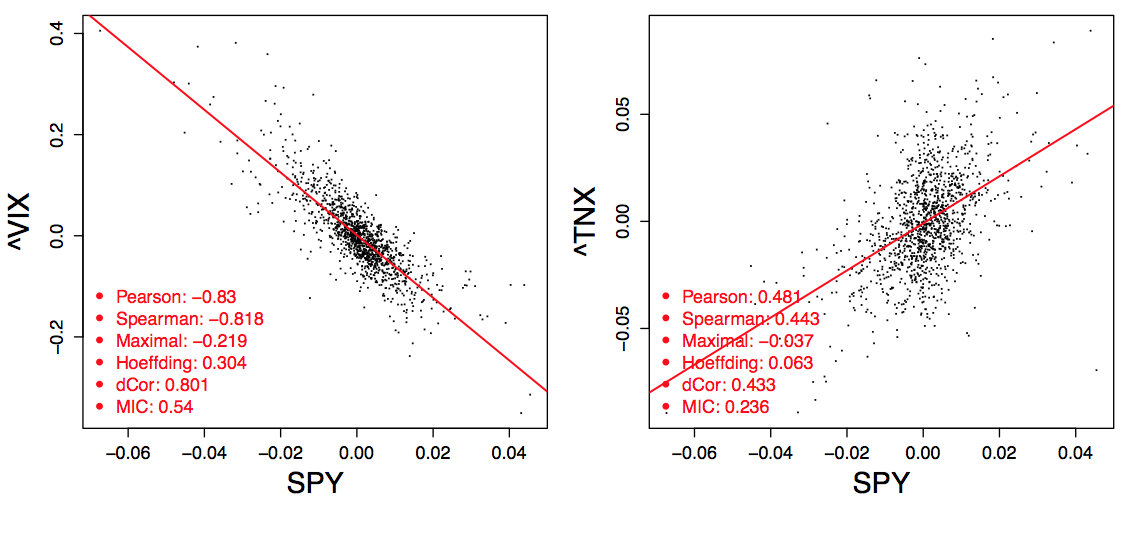
\includegraphics[width=0.7\columnwidth]{pairs_2.png}
\end{center}
\caption{ Analysis of pairs of instruments. 
}
\label{figExample}
\end{figure}

Note regarding submission: there are 8 choose 2 pairs of variables, so please do not print each plot on a full page. In R, when printing to a pdf, you can combine multiple plots on the same graph in a table format, using the command par(mfrow = c(3,5)) ) which prints to table with 3 rows and 5 columns, for example. See for example \url{http://www.statmethods.net/advgraphs/layout.html}

\vspace{3mm}

5) Name a few of the strongest relationships that you observe in (4).

\vspace{3mm}

6) If your goal was to predict future stock returns, and you only had access to the above different types of correlation measures, what would you do to discover variables that affect future returns? Can you give a few simple examples? (Hint: lag, causation). 

\vspace{3mm}

(7) Pick your favorite such new variable, and illustrate it on your favorite pair of instruments. Show your results in a plot similar to the one in Figure \ref{figExample}, where the $y$-axis is the future return of some  instrument A and the $x$-axis is your newly defined variable corresponding to some instrument B.

\vspace{7mm}

Note 1: Please include your code (whatever you add or modify in the existing code) in the homework submission. No need to add my code for scraping the Yahoo data.

Note 2: If you are using a different programming language, the Homework folder contains a csv file with the prices of each of the above instruments. 

Note 3: If you are using a different programming language, and you are not able to find packages for the various above correlation measures, please email me. (I still encourage you to learn R, it can only help you later in your academic/industry career). 

Note 4: The function \texttt{loadYahooData\_saveToFile()} in the R script I provided should be of help later on as well, you can use it to download from Yahoo other financial data. 

Note 5: The function \texttt{test\_correlations} should get you started on the programming assignment. You can always ask any questions you might have along the way. 

\end{document}
 
 ---------------------------------------------------------------------- 